\documentclass{standalone}
\usepackage{tikz}
\usepackage{ctex,siunitx}
\setCJKmainfont{Noto Serif CJK SC}
\usepackage{tkz-euclide}
\usepackage{amsmath}
\usepackage{wasysym}
\usetikzlibrary{patterns, calc}
\usetikzlibrary {decorations.pathmorphing, decorations.pathreplacing, decorations.shapes,}
\begin{document}
\small
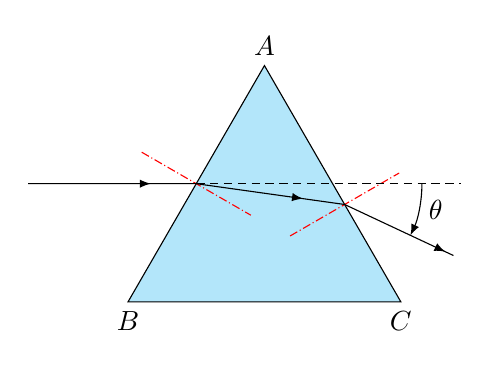
\begin{tikzpicture}[>=latex,scale=1]
  \draw[fill=cyan!30!white](90:2)node[above]{$A$}--(210:2)node[below]{$B$}--(-30:2)node[below]{$C$}--cycle;
  \draw[red,thin,densely dashdotted](150:1.8)--(150:0.2)([shift=(210:0.8)]1.0185,0.236)--++(30:1.6);
  \draw[densely dashed](150:1)--(2.5,0.5);
  \draw[thin,->](2.0,0.5)arc(0:-25.128:1.5445)node[midway,right]{$\theta$};
  \draw[postaction={decorate},decoration={markings,mark=between positions 0.28 and 1.0 step 0.35 with {\arrow{>}}}](-3,0.5)--(150:1.0)--(1.0185,0.236)--(2.4,-0.412);
\end{tikzpicture}
\end{document}